\documentclass[11pt]{article}

\usepackage[margin=1in]{geometry}
\usepackage{amsmath, amssymb}
\usepackage{booktabs}
\usepackage{graphicx}
\usepackage{hyperref}
\usepackage{url}

\title{\textbf{Experimental Report}\\
Scalable Graph Partitioning for Communication-Efficient Distributed Optimization}
\author{Team Members: Name 1, Name 2, Name 3}
\date{CS240: Algorithm Design and Analysis, Spring 2026}

\begin{document}

\maketitle

\section{Background and Related Work}

This project studies graph partitioning as an algorithmic tool for
communication-efficient distributed optimization. In distributed optimization,
large-scale objectives are solved by multiple agents or workers that communicate
through a network. If strongly coupled variables or agents are placed on
different workers, cross-worker communication becomes expensive. A good
partition should therefore keep computational load balanced while minimizing
the number of dependency edges across workers.

Graph partitioning is a classical problem with applications in parallel
scientific computing, sparse matrix computation, distributed graph processing,
and large-scale machine learning. We focus on the balanced $k$-way partitioning
problem. Related methods include spectral partitioning, local-search
refinement, and multilevel graph partitioning. The main reproduced method is
the Kernighan--Lin heuristic, which iteratively improves a partition by moving
or swapping vertices to reduce the cut value. We compare it with spectral
bisection and a greedy balanced baseline.

\section{Representative Method Analysis}

Let $G=(V,E,w)$ be an undirected weighted graph. Each vertex represents a data
block, variable block, agent, or computational task. Each edge represents a
dependency or communication link. Given $k$, the goal is to find disjoint sets
$V_1,\ldots,V_k$ whose union is $V$:
\[
    \min_{V_1,\ldots,V_k}
    \sum_{(u,v)\in E,\;u\in V_i,\;v\in V_j,\;i\neq j} w_{uv},
\]
subject to the balance constraint
\[
    |V_i| \leq (1+\epsilon)\frac{|V|}{k}, \quad i=1,\ldots,k.
\]
The objective models communication across workers, and the balance constraint
models workload distribution.

The greedy baseline assigns vertices one by one to feasible partitions with
low local cut cost. Spectral partitioning forms the graph Laplacian
$L=D-A$, uses the Fiedler vector for bisection, and recursively obtains $k$
parts. The Kernighan--Lin refinement starts from an initial partition and
performs pairwise local-search refinements between partitions. The spectral
method requires an eigen-decomposition; in our implementation this is
$O(n^3)$ for dense matrices, which is acceptable for the course-scale
benchmarks. The greedy baseline is roughly $O(mk)$, and the refinement cost
depends on the number of passes and pairwise subproblems.

\section{Reproduction and Implementation}

The implementation is organized as a Python package under \path{src/}. The
main modules are:
\begin{itemize}
    \item \path{src/graphs.py}: synthetic and small real graph generation;
    \item \path{src/algorithms.py}: greedy, spectral, and Kernighan--Lin methods;
    \item \path{src/metrics.py}: cut weight, normalized cut, and balance ratio;
    \item \path{src/simulation.py}: consensus averaging communication simulation;
    \item \path{src/experiments.py}: benchmark runner and CSV export;
    \item \path{src/plotting.py}: figure generation.
\end{itemize}

The reproduced component is the Kernighan--Lin refinement idea. We use
NetworkX's robust pairwise Kernighan--Lin bisection routine inside a modular
$k$-way refinement loop, initialized by spectral partitioning. This is a
practical adaptation for $k$-way balanced graph partitioning. The experiments
are deterministic with a fixed seed.

\section{Experimental Evaluation}

We evaluate on grid graphs, Erdos--Renyi random graphs, random geometric
graphs, and the Zachary karate club graph. The metrics are cut weight, balance
ratio, runtime, and consensus-related communication. The raw results are saved
to \path{outputs/partition_results.csv}.

Across the benchmark suite, the average cut weights are:
\[
\text{greedy}=98.25,\quad
\text{spectral}=72.75,\quad
\text{Kernighan--Lin}=66.88.
\]
The average cross-partition message counts in the consensus simulation are:
\[
\text{greedy}=15460,\quad
\text{spectral}=11360,\quad
\text{Kernighan--Lin}=10440.
\]
Thus the Kernighan--Lin refinement achieves the lowest average cut and the
lowest average cross-worker traffic. It gives the best cut on six of the eight
graph instances. Spectral partitioning is especially competitive on structured
grid and geometric graphs, where the Fiedler vector captures spatial structure
well.

\begin{figure}[ht]
    \centering
    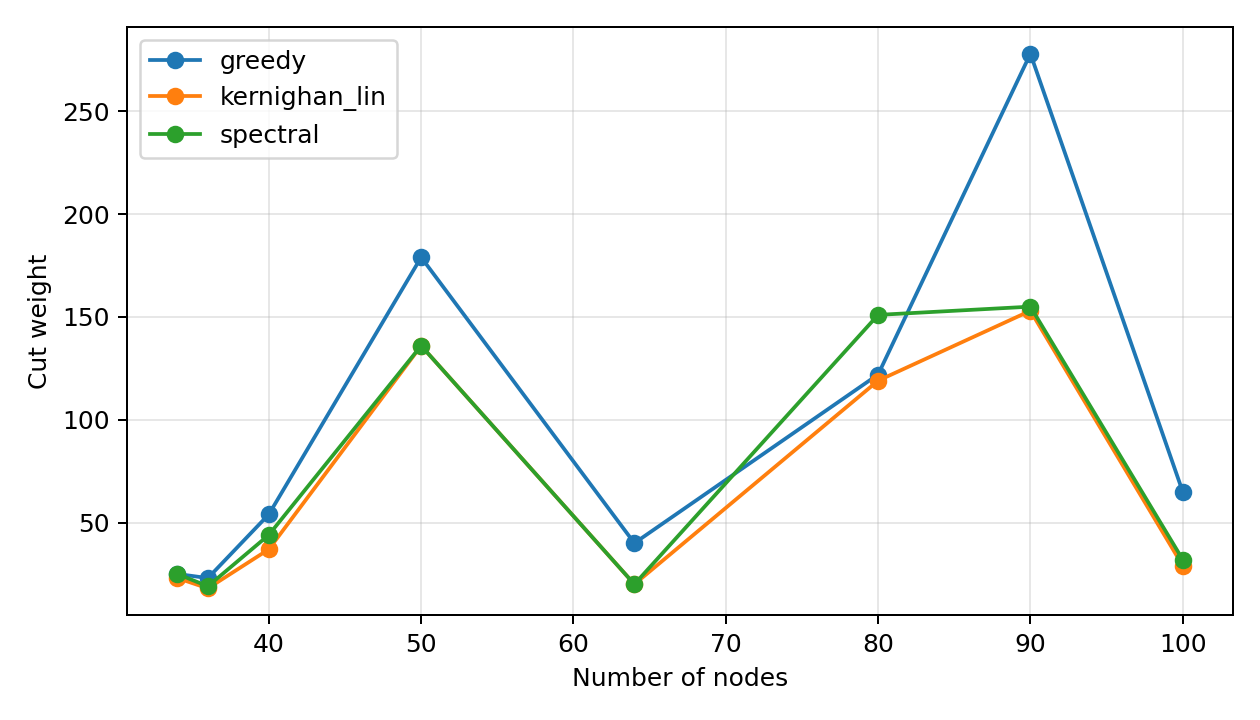
\includegraphics[width=0.75\linewidth]{outputs/figures/cut_weight.png}
    \caption{Cut weight comparison. Lower values indicate less cross-worker
    communication.}
\end{figure}

\begin{figure}[ht]
    \centering
    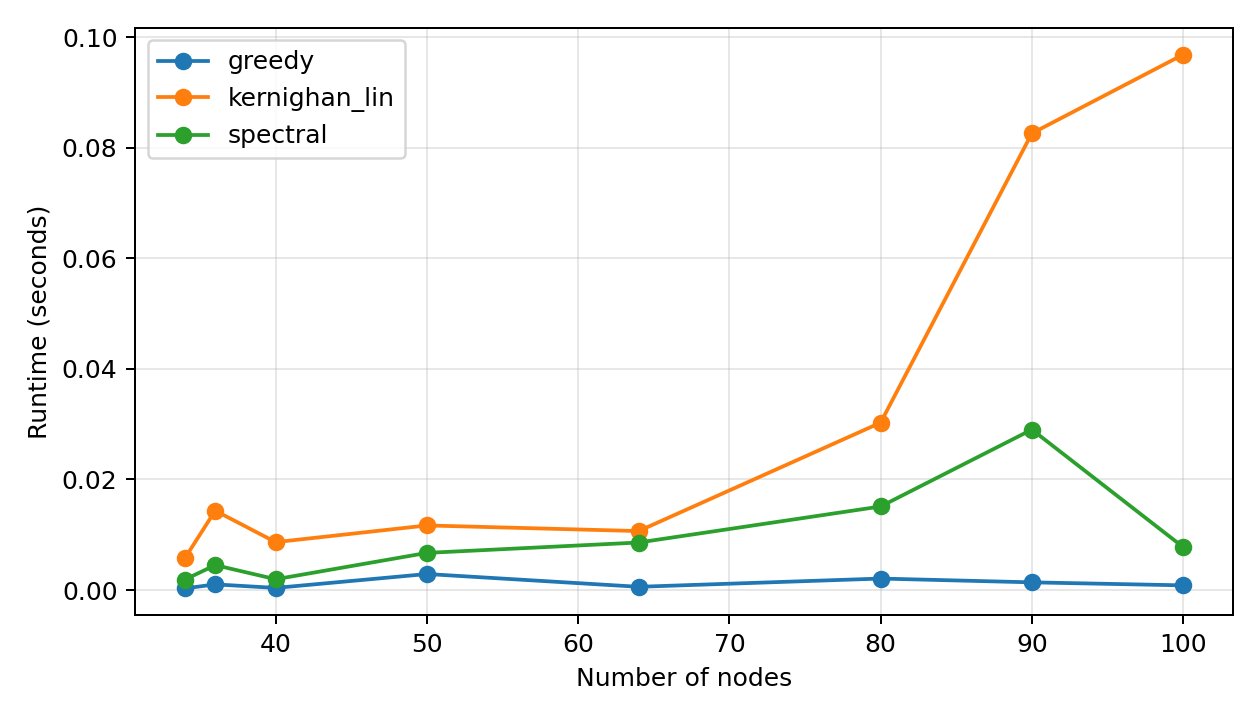
\includegraphics[width=0.75\linewidth]{outputs/figures/runtime_seconds.png}
    \caption{Runtime comparison. The greedy baseline is fastest, while
    Kernighan--Lin spends extra time on refinement.}
\end{figure}

\begin{figure}[ht]
    \centering
    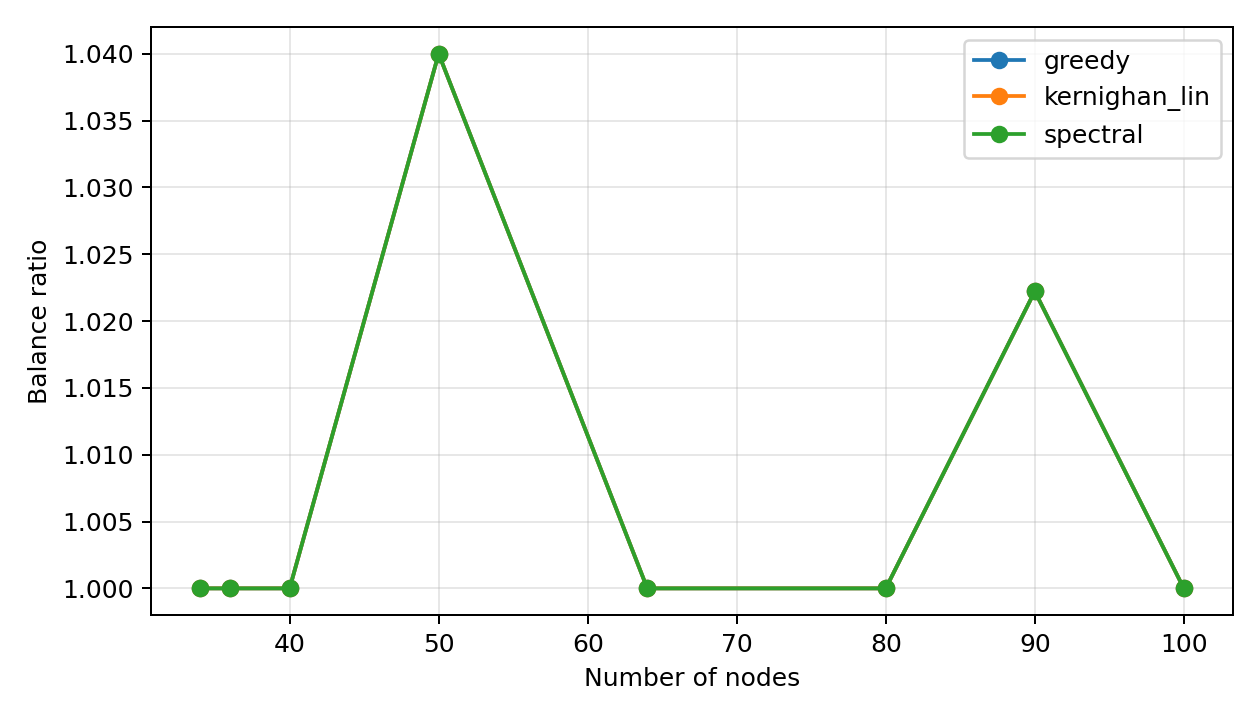
\includegraphics[width=0.75\linewidth]{outputs/figures/balance_ratio.png}
    \caption{Balance ratio comparison. All methods maintain near-balanced
    partitions in the tested cases.}
\end{figure}

The consensus error is almost identical across different partitions on the same
graph, because the simulation keeps the original communication graph fixed and
uses the partition only to count cross-worker traffic. This is expected: the
partition changes communication placement, not the underlying averaging
dynamics. The application-level value of partitioning is therefore reflected
mainly in reduced cross-partition communication cost.

\section{Optional Extension and Discussion}

The current project includes a lightweight distributed optimization simulation
as an extension beyond pure graph partitioning metrics. The main limitation is
that the consensus model does not change the communication topology itself; it
only measures how many messages would cross worker boundaries. A stronger
extension would introduce communication budgets, delayed cross-worker messages,
or weighted communication costs. Another natural extension is to compare with a
full multilevel partitioner such as METIS on larger graphs.

Overall, the experiments support the central claim of the project: classical
graph partitioning algorithms can be used to reduce communication cost in a
modern distributed optimization setting while maintaining balanced workload.

\end{document}
